\documentclass[runningheads,a4paper]{llncs}

\usepackage{amssymb}
\setcounter{tocdepth}{3}
\usepackage{graphicx}
\usepackage[inline]{trackchanges}
\usepackage{subfigure}

\usepackage{url}
\urldef{\mails}\path|{claas.wilke, michael.thiele, c.wende}@inf.tu-dresden.de|
\newcommand{\keywords}[1]{\par\addvspace\baselineskip
\noindent\keywordname\enspace\ignorespaces#1}

% For german character �,�,�,�
\usepackage[latin1]{inputenc}

\begin{document}

\mainmatter  % start of an individual contribution

% first the title is needed

\title{Extending Variability for OCL Interpretation}

% a short form should be given in case it is too long for the running head
\titlerunning{Extending Variability for OCL Interpretation}

% the name(s) of the author(s) follow(s) next
%
% NB: Chinese authors should write their first names(s) in front of
% their surnames. This ensures that the names appear correctly in
% the running heads and the author index.
%
\author{Claas Wilke\and Michael Thiele\and Christian Wende\\
\mails}
%
\authorrunning{Extending Variability for OCL Interpretationn}
% (feature abused for this document to repeat the title also on left hand pages)

% the affiliations are given next; don't give your e-mail address
% unless you accept that it will be published
\institute{Technische Universit�t Dresden\\
Department of Computer Science\\
Institute for Software and Multimedia Technology\\
Software Technology Group
%\url{http://www.st.inf.tu-dresden.de}
}

%
% NB: a more complex sample for affiliations and the mapping to the
% corresponding authors can be found in the file "llncs.dem"
% (search for the string "\mainmatter" where a contribution starts).
% "llncs.dem" accompanies the document class "llncs.cls".
%

\toctitle{Lecture Notes in Computer Science}
\tocauthor{Authors' Instructions}
\maketitle
\note{CW: Are the email addresses correct? Mine is.}
\begin{abstract}
  In recent years, OCL advanced from a language used to constrain UML models to 
  a constraint language that is applied to various object-oriented modelling
  languages. This includes Domain Specific Languages (DSLs) and meta-modelling languages 
  like the Meta Object Facility (MOF) or Ecore. 
  Consequently, it is rather common to provide variability for OCL parsers to
  work with different modelling languages. 
  A second variability dimension relates to the
  technical space that models are realised in. 
  Current OCL interpreters do not support such variability as their implementation 
  is typically bound to a specific technical space like Java,
 Ecore, or a specific model
 repository. In this paper we propose a generic adaptation architecture for OCL
 that hides models and 
% keep model instances to introduce terminology 
 model instances behind well-defined
 interfaces. We present how the implementation of such an architecture for DresdenOCL enables reuse of the same 
  OCL interpreter for various model realisation techniques. Finally, our approach is evaluated in three
  case studies defining and interpreting OCL constraints on multiple models
  and model instances.
  \note{CW: The abstract is too long. 150 words max. allowed!}

\keywords{OCL, OCL Infrastructure, OCL Tool, MDSD, Modelling, Constraint Interpretation, Technological Spaces, Variability, Adaptation.}
\end{abstract}

  \chapter{Getting started with Dresden OCL}
\label{chapter:introduction}

\begin{flushright}
\textit{Chapter written by Claas Wilke and Michael Thiele}
\end{flushright}

This chapter generally introduces into \keyword{Dresden OCL}. Dresden OCL is
based on a \keyword{Pivot Model} developed by Matthias 
Br�uer~\cite{GB:Braeuer} which is shortly explained in 
Chapter~\ref{chapter:architecture}. Further information about Dresden OCL is 
available at the project's website~\cite{WWW:toolkit}.

This chapter explains the installation of Dresden OCL and how to load a 
model, an instance of such a model, and \acs{OCL} constraints defined on such a 
model into Dresden OCL. Besides the Eclipse distribution, Dresden OCL can 
also be used as a stand-alone Java library. If you plan to use the stand-alone 
distribution you can skip this chapter and continue with 
Chapter~\ref{chapter:standalone}. However, this chapter explains the basic 
concepts of Dresden OCL. Although you cannot use the shown GUI wizards and 
browsers when using the stand-alone version, this chapter can be helpful to 
understand the terms used in and the mechanisms provided by Dresden OCL.
  


\section{How to Install Dresden OCL}
	
The following different possibilities exist to install Dresden OCL within
Eclipse.

\begin{enumerate}
	\item You may install Dresden OCL using the \emph{Eclipse Marketplace
	  Client}.
	\item You may install Dresden using the update site available
	  at~\cite{WWW:toolkitUpdatesite},
	\item You may checkout and run the source code distribution from the \acs{SVN}
	  available at~\cite{WWW:toolkitSVN}.
\end{enumerate}

This section will explain all three possibilities.
	

\subsection{Installing Dresden OCL using the Eclipse Marketplace Client}

Since Eclipse 3.6, the new Eclipse Marketplace Client allows easy installation
of Eclipse-based tools such as Dresden OCL.

To install Dresden OCL via the Eclipse Marketplace Client, select the menu
option \emph{Help -> Eclipse Marketplace\ldots}. Probably you have to select a
marketplace catalog afterwards. If so, select the \emph{Eclipse Marketplace}
catalog and proceed.

Type \texttt{Dresden OCL} into the search text field and press the return key.
Select Dresden OCL from the search results and click the \emph{Install} button
(cf. Fig.~\ref{pic:intro:marketplace01}). Afterwards, click through the
installation dialog and Dresden OCL will be installed. Finally you have to 
restart your Eclipse distribution to complete the installation.

\begin{figure}[!b]
	\centering
	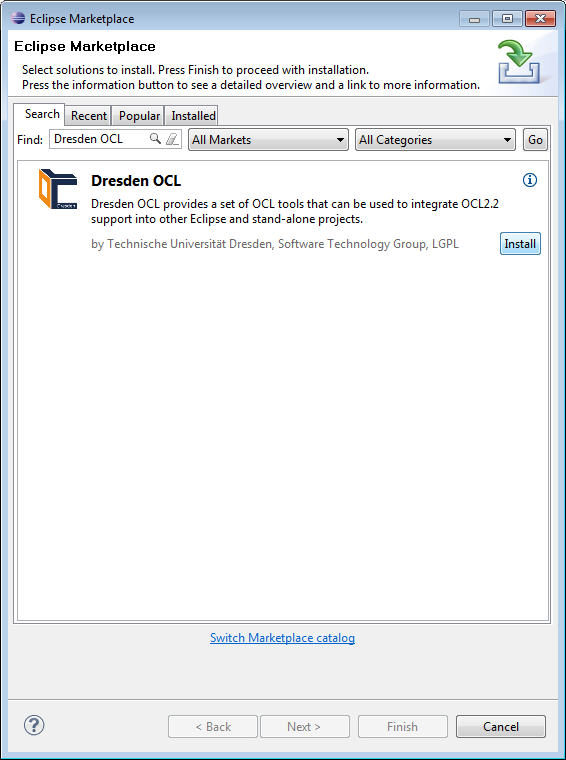
\includegraphics[width=0.8\linewidth]{figures/introduction/marketplace01}
	\caption{Installing Dresden OCL using the Marketplace Client.}
	\label{pic:intro:marketplace01}
\end{figure}


\subsection{Installing Dresden OCL using the Eclipse Update Site}
	
To install Dresden OCL via the \keyword{Eclipse Update Site}, you have to
start an Eclipse instance and select the menu option \eclipse{Help ->
Install New Software\ldots}

Enter the path \url{http://www.dresden-ocl.org/update/} and
click the \eclipse{Add...} button (cf. Fig.~\ref{pic:intro:updateSite01}). 
In the new opened window you can additionally enter a name for the update site 
(cf. Fig.~\ref{pic:intro:updateSite02}).

\begin{figure}[!b]
	\centering
	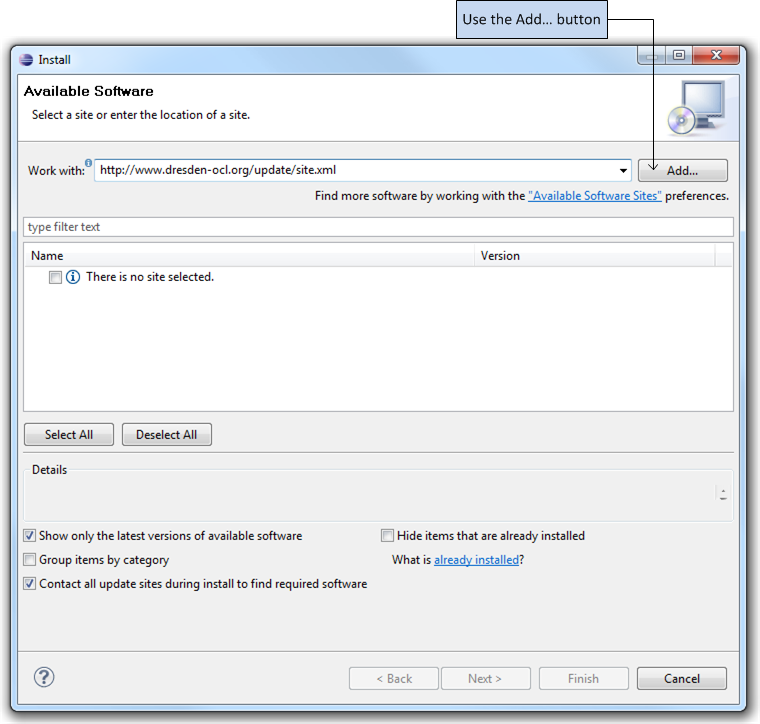
\includegraphics[width=0.8\linewidth]{figures/introduction/updateSite01}
	\caption{Adding an Eclipse Update Site (Step 1).}
	\label{pic:intro:updateSite01}

  \vspace{2.0em}
  
	\centering
	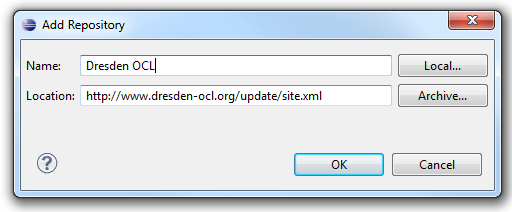
\includegraphics[width=0.6\linewidth]{figures/introduction/updateSite02}
	\caption{Adding an Eclipse Update Site (Step 2).}
	\label{pic:intro:updateSite02}
\end{figure}

Now you can select the features of Dresden OCL which you want to install. 
Select them and click the \eclipse{Next >} button (cf. 
Fig.~\ref{pic:intro:updateSite03}). An overview on all features of 
Dresden OCL can be found in Table~\ref{tab:plugins} in the appendix of 
this manual. Follow the wizard and agree with the user license. Then Dresden OCL
will be installed. Afterwards, you should restart your Eclipse application to 
finish the installation.

\begin{figure}[t]
	\centering
	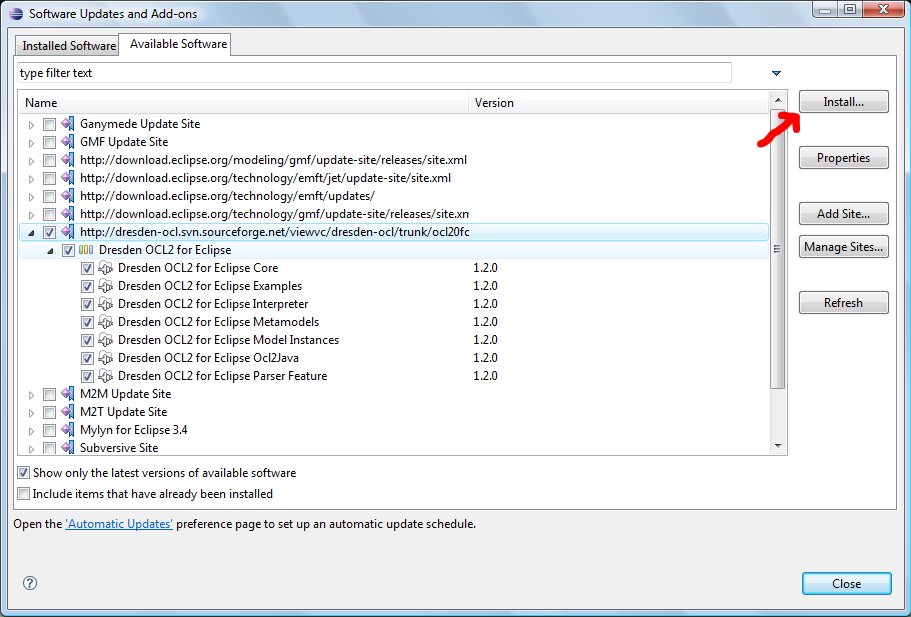
\includegraphics[width=1.0\linewidth]{figures/introduction/updateSite03}
	\caption{Selecting features of Dresden OCL.}
	\label{pic:intro:updateSite03}
\end{figure}
	
	
\subsection{Importing Dresden OCL from the SVN}

To use Dresden OCL by checking out the source code from the \acs{SVN} you
need to install an \acs{SVN} client. In the following the 
\keyword{Eclipse Subversive} plug-in is used.

After installing Eclipse Subversive, a new \keyword{Eclispe Perspective} 
providing access to \acs{SVN} should exist. The perspective can be opened via 
the menu \eclipse{Window > Open Perpective > Other... > SVN Repository
Exploring}. In the view \eclipse{\acs{SVN} Repositories} you can add a new 
repository using the \acs{URL} 
\url{http://svn-st.inf.tu-dresden.de/svn/dresdenocl/} (cf. 
Fig.~\ref{pic:intro:svn01}).

\begin{figure}[!b]
	\centering
	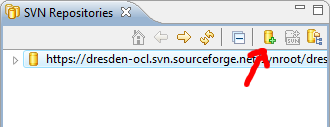
\includegraphics[width=0.4\linewidth]{figures/introduction/svn01}
	\caption{Adding an SVN repository.}
	\label{pic:intro:svn01}
\end{figure}

After clicking the \eclipse{Finish} button, the \acs{SVN} repository root should 
be visible in the \eclipse{\acs{SVN} Repositories} view. To checkout the
plug-ins, you have to select them in the repository directory 
\reference{trunk/ocl20\-for\-Eclipse/eclipse} and use the \eclipse{Checkout...} 
function in the context menu (cf. Fig.~\ref{pic:intro:svn02}).
	
\begin{figure}[!t]
	\centering
	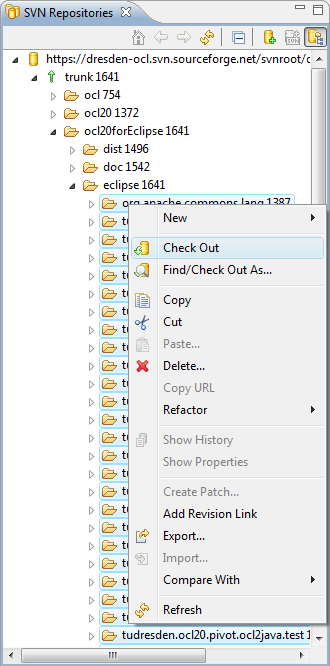
\includegraphics[width=0.4\linewidth]{figures/introduction/svn02}
	\caption{Checkout of Dresden OCL's plug-in projects.}
	\label{pic:intro:svn02}
\end{figure}


\subsection{Problems While Installing Dresden OCL}

Dresden OCL required some other plugins as a prerequesite for its installation. Unfortunately,
the mechanism to declare these dependencies automatically does not work with all installations of
Eclipse well. If during the installation of Dresden OCL problems such as unresolved dependencies occur,
you have to declare these dependent update sites manually.

Open the p2 update manager by the menu option \emph{Help -> Install New Software\ldots}.

Enter the following update sites and confirm each site by pressing the \emph{Add} button:

\begin{itemize}
  \item \url{http://www.emftext.org/update/}
  \item \url{http://download.eclipse.org/tools/ajdt/42/dev/update/}
\end{itemize}

Afterwards, the problem with unresolved dependencies should not occur anymore.


\subsection{Building the OCL2 Parser}
The new Dresden OCL parser/editor is partially written in Scala. In order
to build the sources of the parser without having to have the \reference{Scala
IDE} installed, Dresden OCL comes with various \keyword{Ant} scripts that
compile the Scala code to byte code.

After a checkout, the build script should be called automatically. Be aware that
the compilation might take a while to finish. If other projects that depend on
the parser like the facade still do not compile correctly, try to perform a 
\keyword{refresh} on the plug-ins that contain Scala code.

If the \keyword{Ant} script is not invoked automatically, you can call it either
be cleaning the
\reference{tudresden\linebreak[0].ocl\-20\linebreak[0].pivot.language.ocl.staticsemantics}
plug-in or by running the \keyword{Ant} task \reference{clean all} of the same plug-in.

You have to run the \keyword{ANT} scripts in the same 
\keyword{JRE} as Eclipse. Figures~\ref{pic:intro:parserbuild01} 
and~\ref{pic:intro:parserbuild02} show how to achieve this. If an error like 
``Unable to find javac compiler.'' occurs, you might be trying to run the
\keyword{Ant} script with a \keyword{\acl{JRE}} instead of a \keyword{\acs{JDK}}
(For errors like this one) use the \eclipse{Installed JREs...} button in the
same window to select a \acs{JDK} instead.

If you want to make changes to the static semantics evaluation of the parser you
should consider installing the \emph{Scala IDE} from 
\url{http://www.scala-lang.org/scala-eclipse-plugin}. Be aware that the Scala
code is version 2.7.7 which is not compatible with Scala 2.8 and therefore you
cannot use the current \emph{Scala IDE} which supports only Scala 2.8. 

In order to use the Scala compiler of the IDE, you have to go to the
\eclipse{Properties} of each Scala plug-in, select the tab \eclipse{Builders},
check the \eclipse{Scala Builder} and possibly uncheck the \keyword{Ant} script
for building.

\begin{figure}[p]
	\centering
	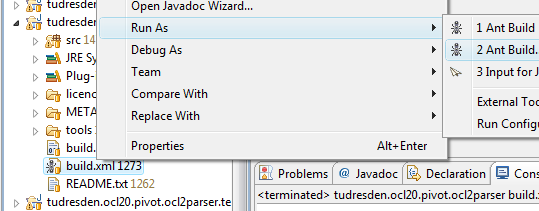
\includegraphics[width=0.8\linewidth]{figures/introduction/parserbuild01}
	\caption{Executing the OCL2 Parser build script.}
	\label{pic:intro:parserbuild01}

  \vspace{4.0em}

	\centering
	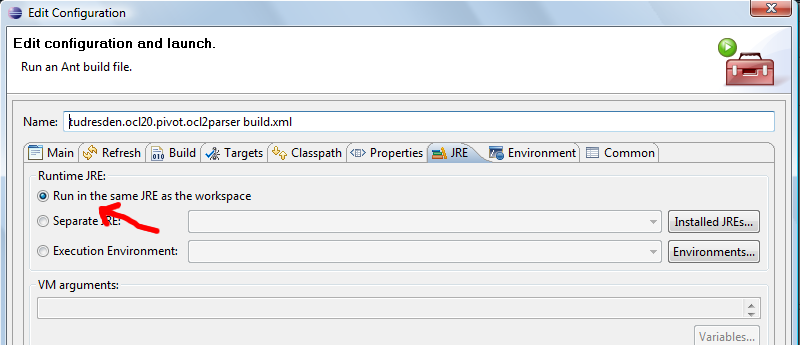
\includegraphics[width=0.8\linewidth]{figures/introduction/parserbuild02}
	\caption{Settings of the JRE for the Ant build script.}
	\label{pic:intro:parserbuild02}

  \vspace{4.0em}

	\centering
	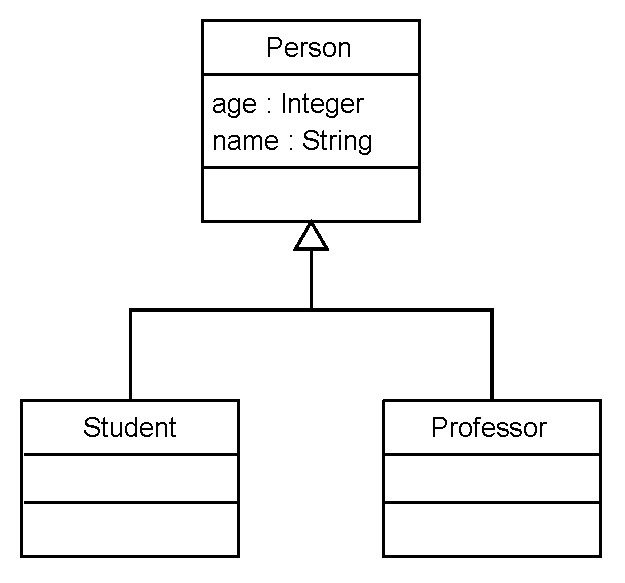
\includegraphics[width=0.5\linewidth]{figures/examples/simple01}
	\caption{A class diagram describing the Simple Example model.}
	\label{pic:examples:simple01}
\end{figure}


\section{Loading Models, Model Instances and Constraints}

If you installed the Dresden OCL using the market place client or update site,
you can execute the toolkit within your Eclipse distribution. If you imported
the Toolkit as source code plug-ins into an Eclipse workspace, you have to start a 
new Eclipse instance. You can start a new instance via the menu \eclipse{Run >
Run As > Eclipse Application}. If the menu \eclipse{Eclipse Application} is not 
available or disabled you need to select one of the plug-ins of the toolkit in
the \eclipse{Package Explorer} first.


\subsection{The Simple Example}
\label{intro:simpleExample}

The use of Dresden OCL is explained using the \keyword{Simple Example} 
which is located in the plug-in 
\reference{tudresden.ocl20.pivot.examples.\linebreak[0]simple}. 
Figure~\ref{pic:examples:simple01} shows a class diagram of the Simple Example.

Dresden OCL provides more examples than the Simple Example. The different 
examples use different metamodels which is possible with the \textit{Pivot
Model} architecture of the Toolkit. An overview on all examples provided 
with Dresden OCL is listed in Table~\ref{tab:examples} in the appendix of
this manual. The Simple Example can be used with two different metamodels. 
These are \keyword{\acs{UML}~2} (based on \keyword{\acs{Eclipse MDT} 
\acs{UML}}) and \keyword{Java}.


\subsection{Dresden OCL Perspective}

Dresden OCL provides its own perspective within Eclipse that contains all views
and editors provided with Dresden OCL. To ease the work with Dresden OCL, you
should now switch to the Dresden OCL perspective. Select the menu option
\eclipse{Window -> Open Perspective -> Other \ldots} and select the perspective
\eclipse{Dresden OCL} (cf. Fig.~\ref{pic:introduction:perspective}).
	
\begin{figure}[!t]
	\centering
	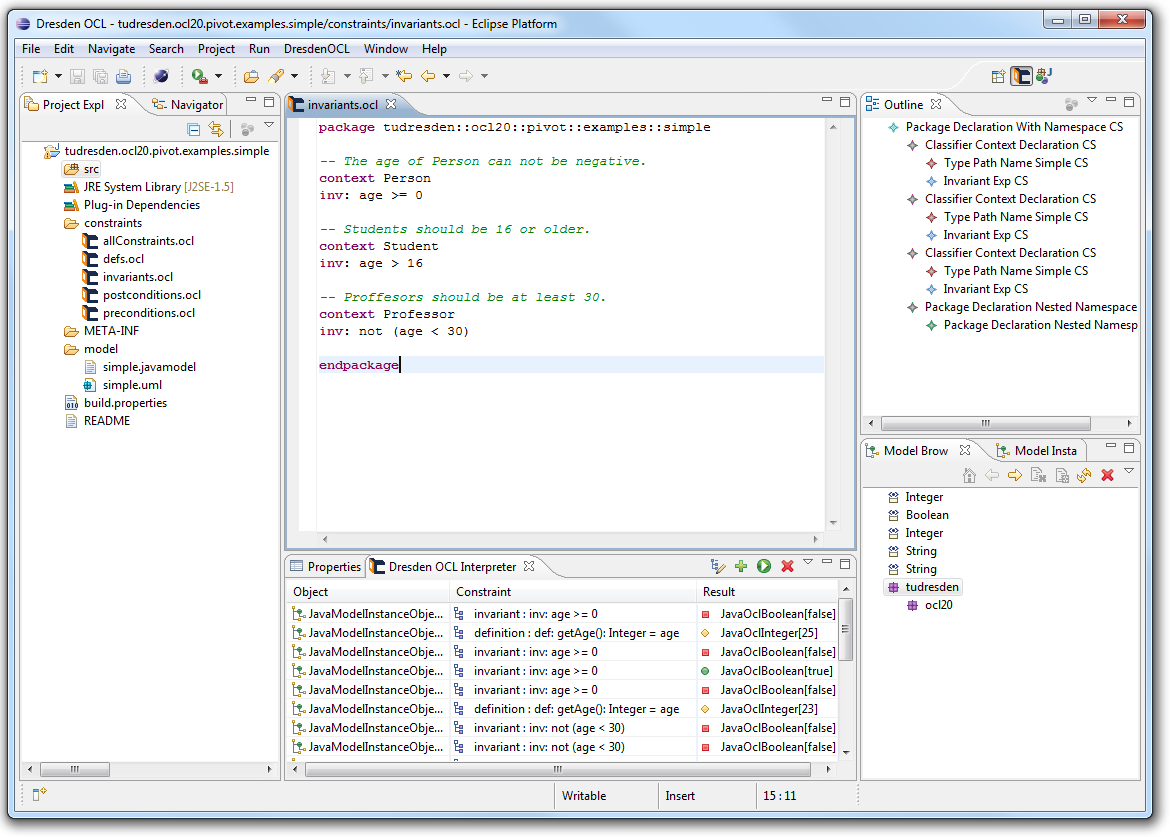
\includegraphics[width=1.0\linewidth]{figures/introduction/perspective}
	\caption{The Dresden OCL Perspective.}
	\label{pic:introduction:perspective}
\end{figure}

On the left hand side the perspective contains the \eclipse{Project Explorer} of
Eclipse to manage different projects. The right hand side contains the
\eclipse{Outline View} for opened \acs{OCL} files. Below, the \eclipse{Model
Browser} and \eclipse{Model Instance Browser} of Dresden OCL allow to explore models and
instances imported into Dresden OCL. At the bottom of the perspective the
\eclipse{OCL Intepreter} is located. The center of the perspective contains the
\eclipse{OCL Editor} of Dresden OCL that allows to edit and parse \acs{OCL}
files for an opened model. How to use the tools provided with Dresden OCL is explained in
the following.


\subsection{Loading a Model}
	
For this tutorial you first have to load a model into Dresden OCL. To ease the
use of the Simple Example project, this project should be imported into the  
\keyword{Workspace} first. Select the menu option \emph{File -> New ->
Other} and select the option \emph{Dresden OCL Examples -> Simple Example}
within the new opened window (cf. Fig~\ref{pic:intro:importexample01}). Click
the \emph{Finish} button to import the project into your workspace. Afterwards, the workspace should contain the Simple
Example project as shown in Figure~\ref{pic:introduction:perspective}, left hand
side.

\begin{figure}[!t]
	\centering
	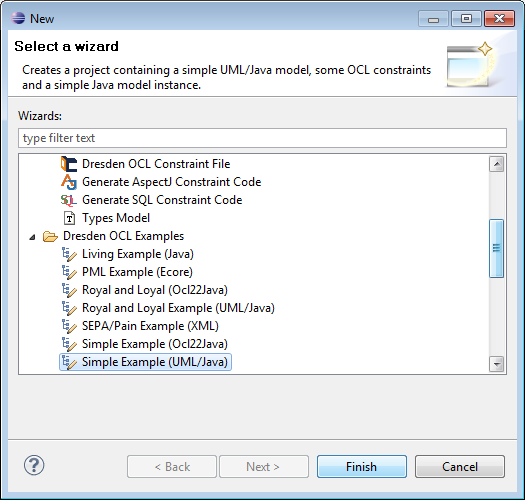
\includegraphics[width=0.8\linewidth]{figures/introduction/importexample01}
	\caption{Importing the Simple Example project.}
	\label{pic:intro:importexample01}
\end{figure}

Now you can import the model into Dresden OCL. Select the
\reference{model/simple.uml} file in the \eclipse{Project Explorer} and open the
context menu (right mouse click). Select the menu option
\eclipse{Dresden OCL > Load Model} (cf. Fig.~\ref{pic:intro:loadmodel00}). In
the opened wizard you have to select the metamodel \acs{UML}2 and click the
\eclipse{Finish} button (cf. Fig.~\ref{pic:intro:loadmodel01}).

Figure~\ref{pic:intro:loadmodel02} shows the imported Simple Example model,
which uses \acs{UML}2 as its meta-model. Via the menu button of the \eclipse{Model 
Browser} (the little triangle in the right top corner) you can switch between 
different models imported into Dresden OCL (cf.  
Fig.~\ref{pic:intro:loadmodel03}). With the two circled arrows icon you can
reload a model into Dresden OCL, with the red \emph{X} you can close the
currently selected model.
	
\begin{figure}[!p]
	\centering
	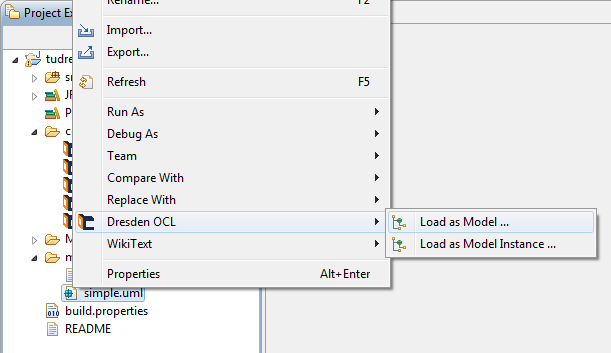
\includegraphics[width=1.0\linewidth]{figures/introduction/loadmodel00}
	\caption{Loading a Model.}
	\label{pic:intro:loadmodel00}
	
  \vspace{6.0em}
	\centering
	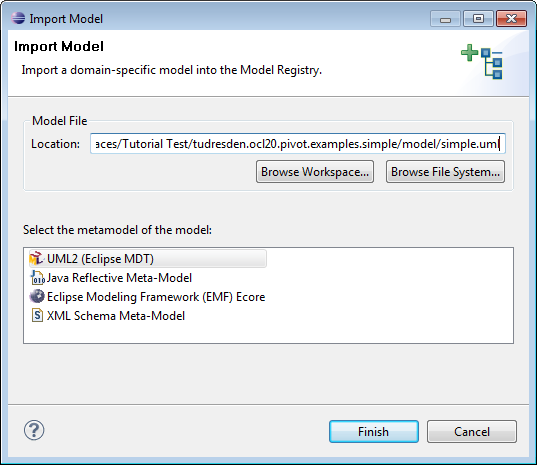
\includegraphics[width=0.7\linewidth]{figures/introduction/loadmodel01}
	\caption{Loading a Model.}
	\label{pic:intro:loadmodel01}
\end{figure}
	
\begin{figure}[!p]
	\centering
	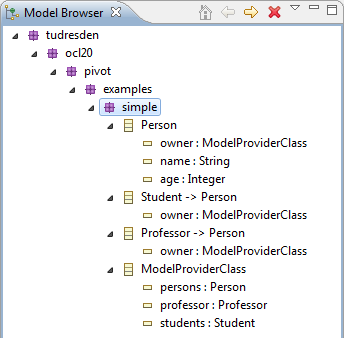
\includegraphics[width=0.4\linewidth]{figures/introduction/loadmodel02}
	\caption{The Simple Example model within the Model Browser.}
	\label{pic:intro:loadmodel02}
	
	\vspace{6.0em}

	\centering
	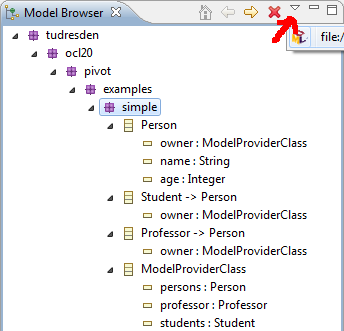
\includegraphics[width=0.4\linewidth]{figures/introduction/loadmodel03}
	\caption{You can switch between different Models using the little triangle.}
	\label{pic:intro:loadmodel03}
	
\end{figure}

	
\subsection{Loading a Model Instance}
\label{intro:loadModel}

After loading a model, you can load an instance of this model using another 
wizard. The model instance is required to interpret \acs{OCL} constraints on
elements instantiating the classes described in the opened model. Which kinds
of model instances are supported in Dresden OCL is documented in
Section~\ref{sect:info:modelinstances}. 
Since the Simple Example provides a Java model instance, we now have to select a
\code{*.java} or \code{*.class} file. Select the file
\reference{src/tudresden/ocl20/\linebreak[0]pivot/examples/\linebreak[0]sim\-ple/\linebreak[0]in\-stance/\linebreak[0]Mo\-del\-InstanceProviderClass\linebreak[0].java}
of the Simple Example in the \eclipse{Project Explorer}. Open the context menu 
and select the menu option \eclipse{Dresden OCL > Load Model Instance} (cf.
Fig.~\ref{pic:intro:loadInstance00}).
In the opened wizard you have to select a model for which the model instance 
shall be loaded and the type of model instance you want to load (cf.
Fig.~\ref{pic:intro:loadInstance01}). Select the \keyword{Java Instance} type
and click the \eclipse{Finish} button.

\begin{figure}[!p]
	\centering
	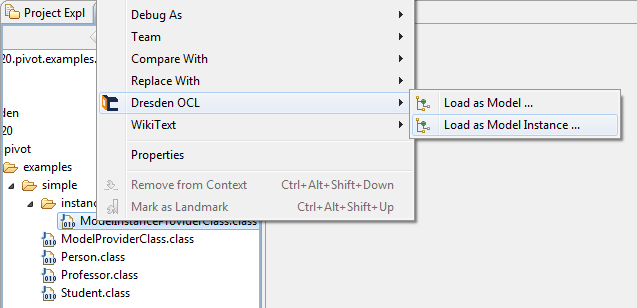
\includegraphics[width=0.7\linewidth]{figures/introduction/loadinstance00}
	\caption{Loading a Simple Model Instance.}
	\label{pic:intro:loadInstance00}

  	\vspace{6.0em}
  
	\centering
	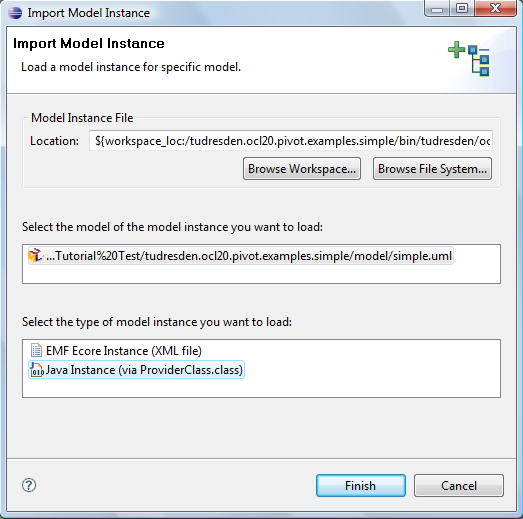
\includegraphics[width=0.7\linewidth]{figures/introduction/loadinstance01}
	\caption{Loading a Simple Model Instance.}
	\label{pic:intro:loadInstance01}
\end{figure}

Figure~\ref{pic:intro:loadInstance02} shows the imported model instance. Like
in the model browser you can switch between different model instances and you 
can close selected instances. Note that the \eclipse{Model Instance Browser} 
only shows the model instances of the model actually selected in the model 
browser. By switching the model in the model browser, you also switch the pool 
of model instances available in the model instance browser.

\begin{figure}[!p]
	\centering
	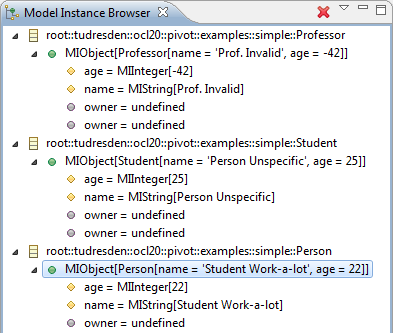
\includegraphics[width=0.6\linewidth]{figures/introduction/loadinstance02}
	\caption{A simple model instance in the Model Instance Browser.}
	\label{pic:intro:loadInstance02}

	\vspace{4.0em}
	
	\centering
	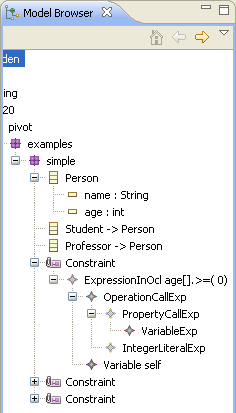
\includegraphics[width=0.4\linewidth]{figures/introduction/loadconstraints02}
	\caption{Parsed expressions and the model in the Model Browser.}
	\label{pic:intro:loadconstraints02}
\end{figure}
	
	
\subsection{Parsing OCL Expressions}
\label{intro:oclEditor}
Any file with the file extension \texttt{.ocl} can be opened with the
\keyword{Dresden OCL Editor}. Once opened, syntactic checks are performed
to analyse whether the given file contains valid \acs{OCL} code. If currently
there is no active model selected in the \eclipse{Model Browser}, the editor
will fail to perform the static semantics analysis and will yield that there is
no active model. You can load a model and then re-parse the \acs{OCL} file by
changing the \acs{OCL} file (e.g., by introducing and immediately deleting a
whitespace character).

The editor/parser will automatically add parsed constraints to the
model as well as \keyword{definitions} to the appropriate
classes. You can inspect the changes on the model in the \eclipse{Model
Browser}. Note that the \keyword{definitions} and constraints are not added to
your model -- they belong to the view of Dresden OCL on the model. The result
can be seen in Figure~\ref{pic:intro:loadconstraints02}. You also can remove
parsed constraints from the model which is shown in
Figure~\ref{pic:intro:loadconstraints03}.

\begin{figure}[t]
	\centering
	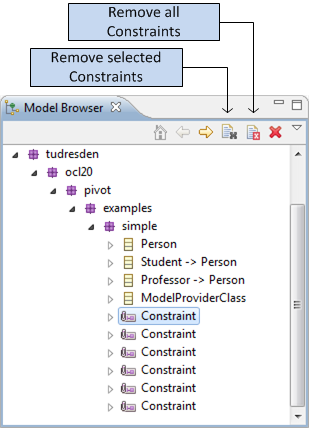
\includegraphics[width=0.4\linewidth]{figures/introduction/loadconstraints03}
	\caption{How to remove Constraints from a Model again.}
	\label{pic:intro:loadconstraints03}
\end{figure}


\subsection{Referencing the constrained Model}

The architecture of Dresden OCL requires that a model must always be imported before
a constraint file can be parsed correctly. Thus, if a constraint file is opened before
its model has been loaded, its complete contend will be marked as erroneous, as the
OCL parser is not able to resolved the referenced files.

To avoid this situation, an annotation can be added to an OCL file that references to
the constraint model specifying a relative path to the model file. The annotation must
be included in a comment at the top of the OCL file consisting of the pattern
\texttt{@model{<path>}} (e.g., for the constraint files of the simple example, the annotation
\texttt{@model{../model/simple.uml}} should work).


\subsection{Refactorings for Dresden OCL}

Dresden OCL can be extended with support for OCL refactorings to ease and improve OCL editing.
How refactorings can be installed and used in Dresden OCL is shortly explained in the following.

\subsubsection{Installation of Refactorings for Dresden OCL}

\begin{itemize}
  \item Install Refactory from the following URL: \url{http://www.emftext.org/update/}.
  \item Install the Refactoring for Dresden OCL feature from: 
  \url{http://www.modelrefactoring.org/DresdenOCLRefactoring/} 
\end{itemize}

\subsubsection{Usage of OCL Refactorings}

After installing the refactoring support, refactorings can simply be performed by selecting
an element in the OCL editor, opening the context menu and select the respective refactoring
(e.g., you can extract a variable as shwon in Fig.~\ref{pic:intro:refactoring01}--\ref{pic:intro:refactoring03}).

\begin{figure}
	\centering
	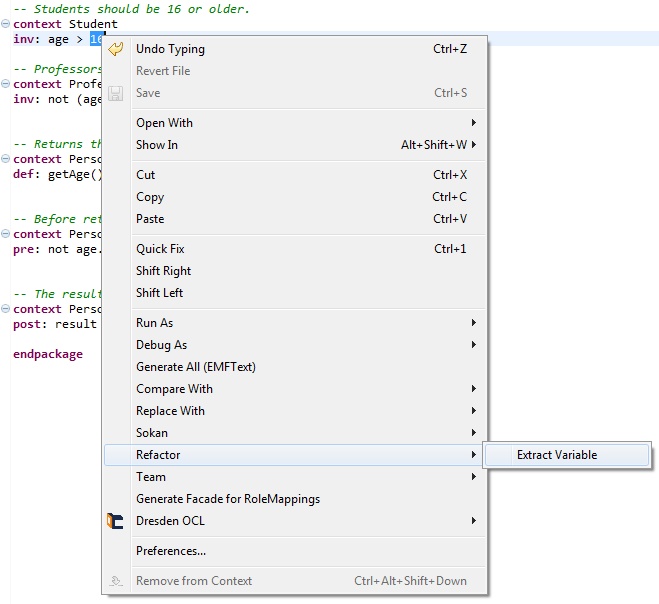
\includegraphics[width=0.35\linewidth]{figures/introduction/refactoring01.png}
	\caption{Extracting a variable: issue the refactoring.}
	\label{pic:intro:refactoring01}

	\vspace{2.0em}
	
	\centering
	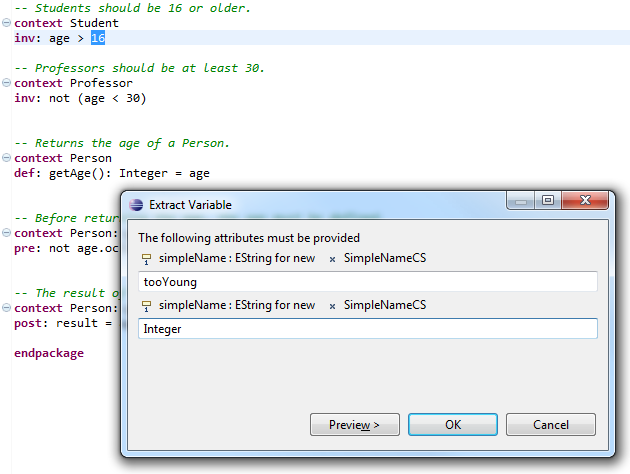
\includegraphics[width=0.8\linewidth]{figures/introduction/refactoring02.png}
	\caption{Extracting a variable: enter parameters.}
	\label{pic:intro:refactoring02}

	\vspace{2.0em}

	\centering
	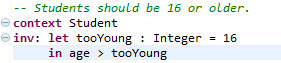
\includegraphics[width=0.35\linewidth]{figures/introduction/refactoring03.png}
	\caption{Extracting a variable: the result.}
	\label{pic:intro:refactoring03}
\end{figure}
	

\section{Possible Use Cases of Dresden OCL using different Models and Model
Instances}
\label{sec:usecases}

Dresden \acs{OCL} can be used in the context of different kind of models and
instances and even at different modeling layers. This section tries to name some 
prominent examples for possible use cases of Dresden \acs{OCL} w.r.t.
different kinds of models and instances. Readers who are not interested in
these details are encouraged to skip this section.

In general, Dresden \acs{OCL} supports the use of \acs{OCL} at two different 
levels: First, \acs{OCL} constraints can be defined on a metamodel and evaluated
on instances of this metamodel (i.e., models). In this context,
\acs{OCL} constraints are often called \emph{\acf{WFRs}}. Second, \acs{OCL}
constraints can be defined on a model and evaluated on instances of this model
(i.e., runtime objects or data). These constraints are often called
\emph{\acf{BRs}}. Examples for both use cases are shown in
Table~\ref{tab:usecases} and shortly explained in the following.

\begin{table}[!t]
\begin{tabular}{|p{7cm}p{7cm}|}
  \hline
  \textbf{WFR Specification and Evaluation} & \\
  \hline
  EMF/Ecore-based model,\newline e.g., \texttt{mydsl.ecore} &
  EMF/Ecore-based instance (model),\newline e.g., \texttt{model01.mydsl} \\
  \hline
  UML metamodel,\newline \texttt{uml.ecore} of MDT/UML &
  UML instance (model),\newline e.g., \texttt{model01.uml} \\
  \hline
  \hline
  \textbf{BR Specification and Evaluation} & \\
  \hline
  UML-based model,\newline e.g., \texttt{model01.uml} &
  Java-based instance (runtime objects),\newline e.g., \texttt{Instance01.java}
  \\
  \hline
  Java classes,\newline e.g., \texttt{Model01.java} &
  Java-based instance (runtime objects),\newline e.g., \texttt{Instance01.java}
  \\
  \hline
  XML Schema (\acs{XSD}),\newline e.g., \texttt{mySchema.xsd} &
  XML instance (data),\newline e.g., \texttt{Instance01.xml} \\
  \hline
\end{tabular}
\caption{Different possible use cases of Dresden OCL.}
\label{tab:usecases}
\end{table}


\subsection{Use Cases of Dresden OCL for Well-Formedness Rules}

Dresden \acs{OCL} supports different scenarios, where \acs{OCL} rules can be
specified on metamodels as \acs{WFRs}. The mose prominent scenarios are shortly
explained below.

\subsubsection{WFRs for EMF/Ecore Models} 
\acs{EMF}/Ecore is often used as a metamodeling language to develop \acl{DSL}s
(\acs{DSL}s). To specify \acs{OCL} constraints on an Ecore-based metamodel, you
import the model file (e.g., \texttt{mydsl.ecore}) as a model into Dresden
\acs{OCL} using the model importer for \acs{EMF}/Ecore-based models. Afterwards,
you can specify \acs{OCL} constraints using the \acs{OCL} parser/editor of
Dresden \acs{OCL}. You can import istances of your \acs{DSL} into Dresden
\acs{OCL} using the model instance importer for \acs{EMF}/Ecore-based instances
(e.g., \texttt{model01.mydsl}) to interpret the specified constraints on them.

\subsubsection{WFRs for the UML Metamodel}
Another common use case is the specification of \acs{OCL} constraints on the
\acs{UML} metamodel and their evaluation for instances of the metamodel (i.e.,
\acs{UML} models). You can do this by importing the \acs{EMF}/Ecore-based
\acs{UML}-metamodel of the Eclipse \acf{MDT}. You can find the required
\texttt{uml.ecore} within the Eclipse plug-in \texttt{org.eclipse.uml.uml} of
Eclipse MDT. Please note, when importing this metamodel into Dresden \acs{OCL},
you have to import it using the \acs{EMF}/Ecore model importer and not a
\acs{UML} model importer (since the \acs{UML} metamodel was modelled in \acs{EMF})!
Afterwards, you can import a \acs{UML} model as an instance of the metamodel to
evaluate constraints on it (e.g., \texttt{model.uml}). Again, you have use
the \acs{EMF}/Ecore model instance importer.


\subsection{Use Case of Dresden OCL for Busines Rules}

Besides the evaluation of \acs{WFRs}, multiple use cases for the evaluation of
\acf{BRs} are supported and explained below.

\subsubsection{BRs for UML models}
A common use case is the definition of \acs{OCL} constraints on a \acs{UML}
model (e.g., \texttt{model01.uml}), typically containing a class model. You can
import \acs{UML} class models into Dresden \acs{OCL} using the corresponding
model importer. For \acs{OCL} evaluation a
possible model instance is a set of runtime objects by using a Java class and
the Java model instance importer (e.g., \texttt{Instance01.java}). Details how
a Java class usable as a Java model instance must be implemented are documented
in Section~\ref{subsec:javaInstance}.

\subsubsection{BRs for Java Classes}
Another possible use case is the use of a set of Java classes as a model for
\acs{OCL} constraint specification (e.g., \texttt{Model01.java}). A Java class
can be imported as a model using the Java model importer. Details how the class
is imported as a model are documented in Section~\ref{subsec:javaModel}. Again,
a typical model istance would be a set of Java objects as mentioned above
(e.g., \texttt{Instance01.java}).

\subsubsection{BRs for XML Schemata}
Dresden \acs{OCL} supports the definition of \acs{OCL} rules on \acl{XSD}s
(\acs{XSD}s) as well (e.g., \texttt{mySchema.xsd}) using the \acs{XSD} model
importer. Obviously an \acs{XML} file would be an appropriate model instance,
using the \acs{XML} model instance importer (e.g., \texttt{Instance01.xml}).


\subsection{Further Use Cases}

Of course, the use cases presented above are not a complete list of all possible
use cases. Theoretically, every supported type of model importer can be combined
with every type of model instances. And besides, you can even define your own
importers for further use cases, if necessary. How to adapt Dresden \acs{OCL} to
other types of models and instances is documented in the
Chapters~\ref{chapter:pivotModelAdaptation}
and~\ref{chapter:modelInstanceTypeAdaptation}.



\section{Summary} 

This chapter described how to use Dresden OCL. It was explained how to 
install the plug-ins of Dresden OCL. Afterwards, the import of models,
model instances and \acs{OCL} constraints into Dresden OCL was explained.

Now, the imported models can be used with the tools provided by Dresden OCL. For
example you can use the \keyword{OCL Interpreter} to interpret \acs{OCL} 
constraints for a given model and model instance (as explained in 
Chapter~\ref{chapter:interpretation}) or you can use the \keyword{OCL22Java
Code Generator} to generate \keyword{AspectJ} code for a loaded model and 
\acs{OCL} constraints (as explained in Chapter~\ref{chapter:codeGeneration}).
How the \keyword{OCL2SQL Code Generator} can be used to generated SQL schema and
integretiy views is documented in Chapter~\ref{chapter:ocl2sql}.

If you do not want to use Eclipse, but still want to interpret OCL constraints 
or generate AspectJ code, you can use Dresden OCL as a stand-alone library
outside of Eclipse. A detailed description on how to do this is given in 
Chapter~\ref{chapter:standalone}.
   
  \section{The Generic Architecture of Dresden OCL2 for Eclipse}
	\note{First motivate variation, adapt section heading accordingly}

		\begin{figure}[tb]
			\centering
				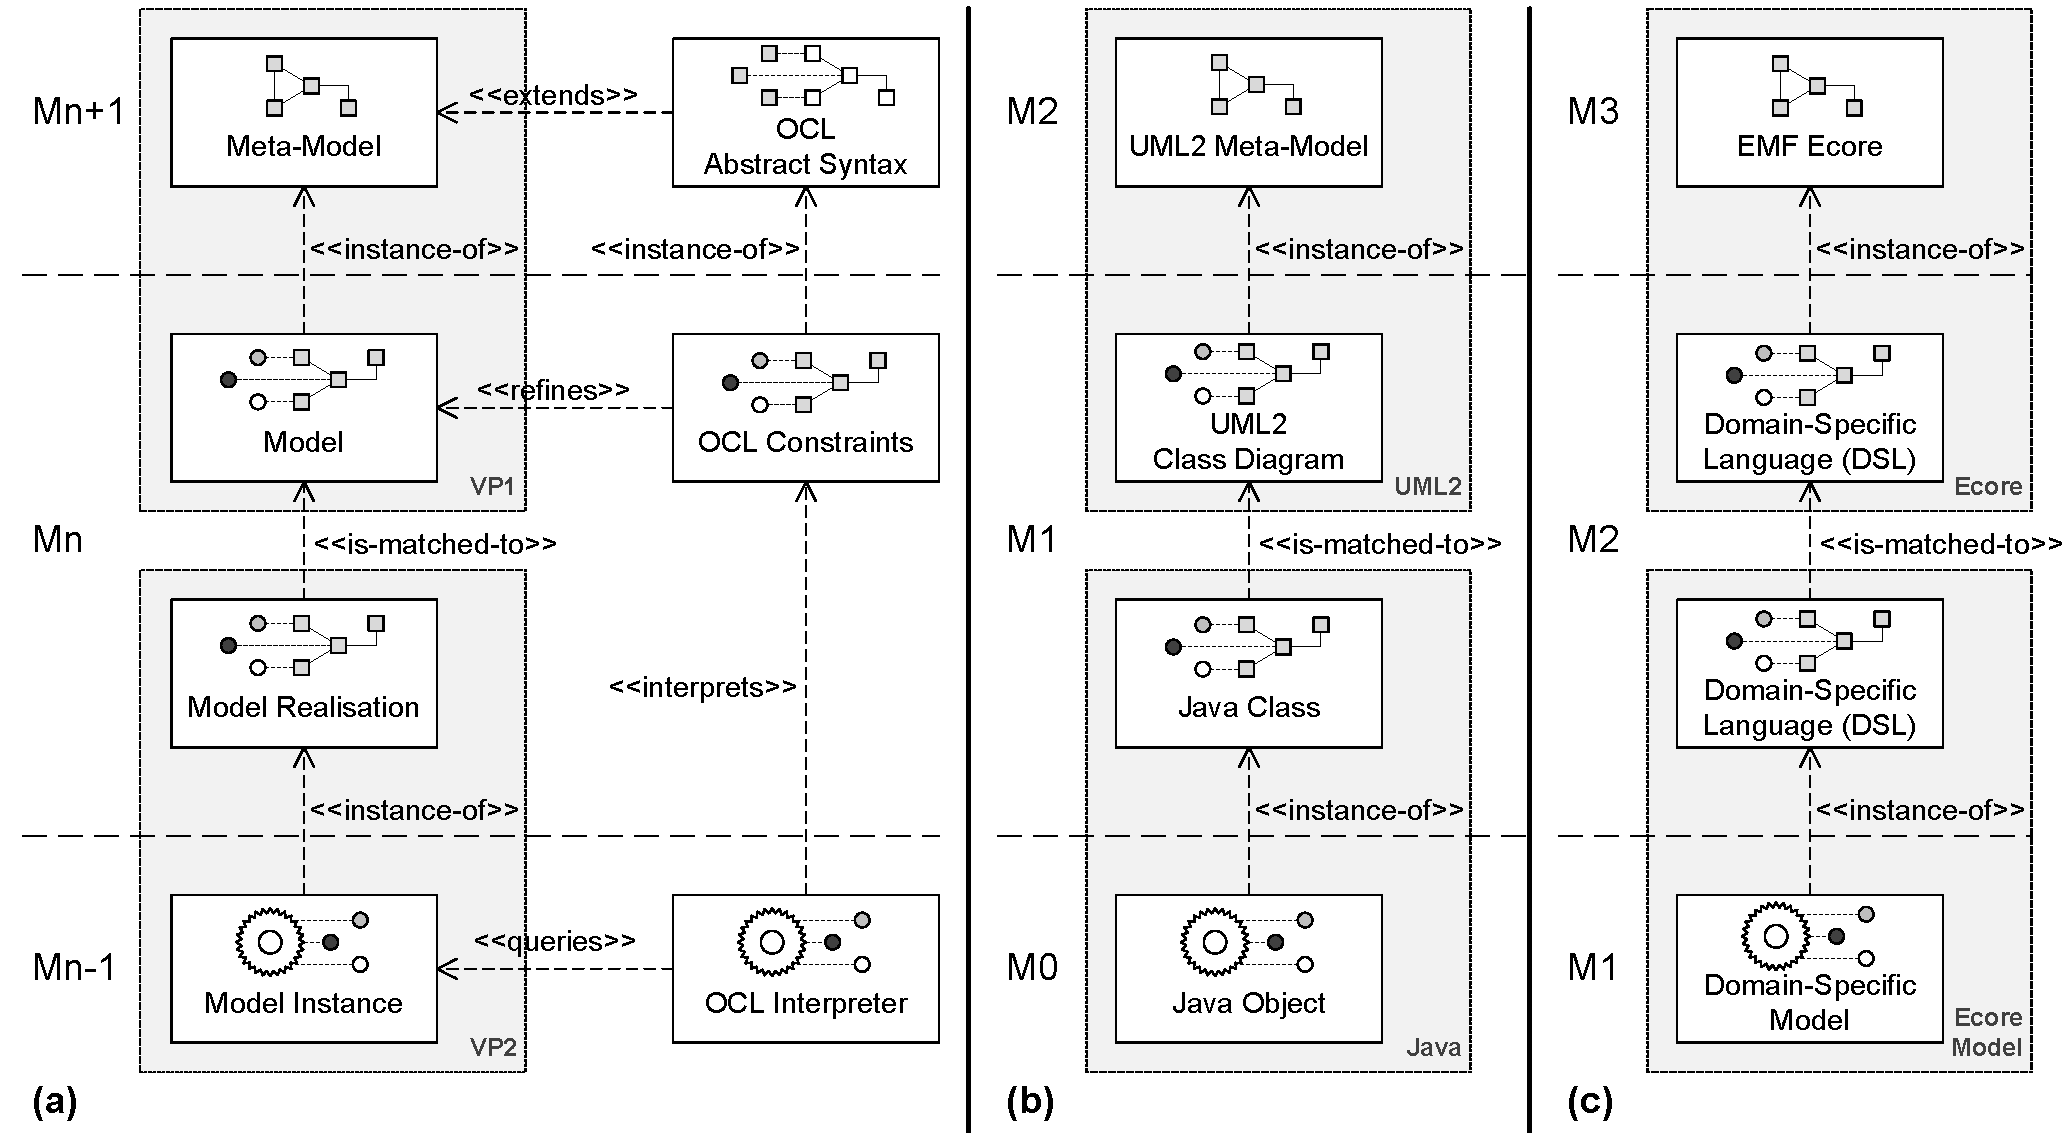
\includegraphics[width=1.00\textwidth]{figures/genericlayers.pdf}
			\caption{\note{Michael: still too much caption text; in (b), is the UML2 meta-model really MOF?, I thought MOF is on M3} The \textit{Generic Three Layer Meta data Architecture}. (a): Each OCL constraint 
			requires a meta-model defining a model on which OCL constraints are specified. The 
			constraints are evaluated on a model instance that instantiates the constrained model. 
			The generic architecture can be parametrized at two different variation points. Different
			models and their meta-models can be bound to VP1, different model instances can be bound
			to VP2.	(b): UML-Example for layers M2, M1 and M0. VP1 is bound to the UML meta-model (MOF), 
			VP2 is bound to Java. (c): EMF-Example for layers M3, M2 and M1. VP1 is bound to EMF Ecore,
			VP2 is bound to Ecore-based models.}
			\label{fig:genericlayers}
		\end{figure}

	To differentiate between meta-models, models and runtime objects, the OMG introduced 
	the \textit{MOF Four Layer Metadata Architecture}, that locates the meta-model, 
	model, and the model's instances at the layers \textit{M2}, \textit{M1} and \textit{M0}. 
	\note{Is that important to understand the paper?; Michael: agreed, just refer to it, but leave explaination}{Each language at layer
	\textit{Mn} is described in terms of a language resided at layer \textit{Mn-1}. Meta-meta-models 
	that are located at the layer \textit{M3} 
	can describe themselves reflexively.}
	
	Fig.~\ref{fig:genericlayers} depicts the \textit{Generic Three Layer
	Meta-Data Architecture} aligning OCL constraints with the MOF layers.
	\remove{As all
	models can be located in this layer architecture, OCL can be located there as
	well.} OCL constraints are a model and can be described using their abstract
	syntax, i.e., the OCL meta-model. They are evaluated for runtime objects at the 
	model instance layer. 
	%\remove{Thus, three layers must be known by the OCL tool
	%to define and evaluate the constraints. This notion leads to the 
	%Generic Three Layer Meta-Data Architecture demuthRGWS09} that 
	%allows to define an OCL tool independently of specific layers. As can be seen
	%in Figure \ref{fig:genericlayers} the OCL model (all constraints) enriches
	%another model.} 
	In order to \change{navigate through the  model or to call
	operations on}{define constraints on models OCL needs to navigate on} model
	elements. To bind OCL constraints on the navigation structure in
	the model they are defined on, the abstract syntax of OCL
	\note{this is true for UML, but sounds quite technical}{extends} the model's
	meta-model.
	%OCL can be used to define well-formedness rules, i.e., constraints on meta-models (M2) that are evaluated at the model level (M1), or business rules, i.e., constraints defined on models (M1) that are evaluated for runtime objects at the model instance layer (M0).
	
	\note{we need to incorporate the motivation for implementation language
	variation here. Reviewers need to understand the problem to understand our
	solution.}


	\note{This section does not clarify the contribution of THIS paper. We should
	sell the instance adaptation as a improvement of previous DresdenOCL versions

		\begin{itemize}
		  \item motivation: different model implementations are useful
		  \item context: identify variation points in fig 1, modeling langauge,
		  implementation language
		  \item problem: neither dresdenOCL nor others are able to cope with differnt
		  model implementations
		  \item solution: we suggest additional adaptation interface
		  \item feasibility: we contribute implementation of adaptation approach in
		  Dresden OCL
		\end{itemize}
	
	}

	{The architecture of Dresden OCL2 for Eclipse was developed in respect to the 
	generic three layer meta-data architecture. In order to reuse the developed 
	OCL tools, DresdenOCL does not directly accesses models or model instance objects. 
	Instead, these are hidden behind a common set of interfaces that delegate to 
	their adaptee. The adaption of models and model instance objects is presented 
	in the following.}


  \section{Implementation}

	In this section we discuss the suggested solution to provide a \emph{Generic Adaptation Architecture} for 
	meta-model, model and model instance independent OCL interpretation. First, we present the solution addressing
	the first variation point of an OCL infrastructure (VP1) to
	adapt	various meta-models and models summarized as \emph{Model Adaptation}. Afterwards, we move the approach
	from the meta-model (Mn+1) to the model (Mn) layer to address the second variation point (VP2) and to support 
	generic \emph{Model Instance Adaptation} as well.
	
	\begin{figure}[!t]
			\centering
				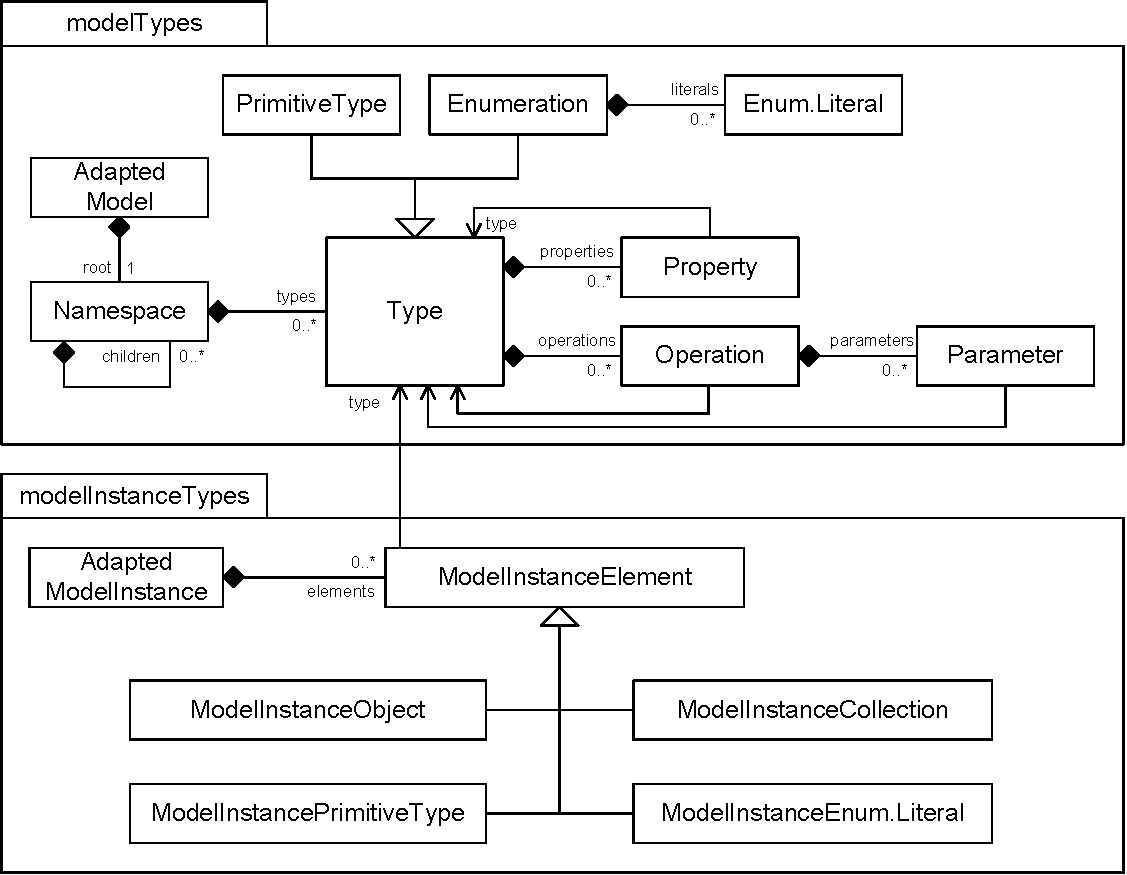
\includegraphics[width=0.80\textwidth]{figures/coreconcepts.pdf}
			\caption{The core concepts of the \emph{Model Types} and \emph{Model Instance Types}:
			Each \emph{Model} has a root \emph{Namespace} that contains a set of nested Namespaces and 
			a set of \emph{Types}. Each Type has a set of \emph{Operations} 
			and \emph{Properties}. 
			Each \emph{Model Instance} has a set of \emph{Model Instance Elements}. Each Model Instance
			Element has exactly one Type and provides 
			operations to reflect on this Type. \emph{Model Instance Objects} provide further reflective 
			operations to get properties and to invoke operations.}
			\label{fig:coreconcepts}
		\end{figure}

\subsection{Model Adaptation}

	\begin{figure}[!t]
			\centering
				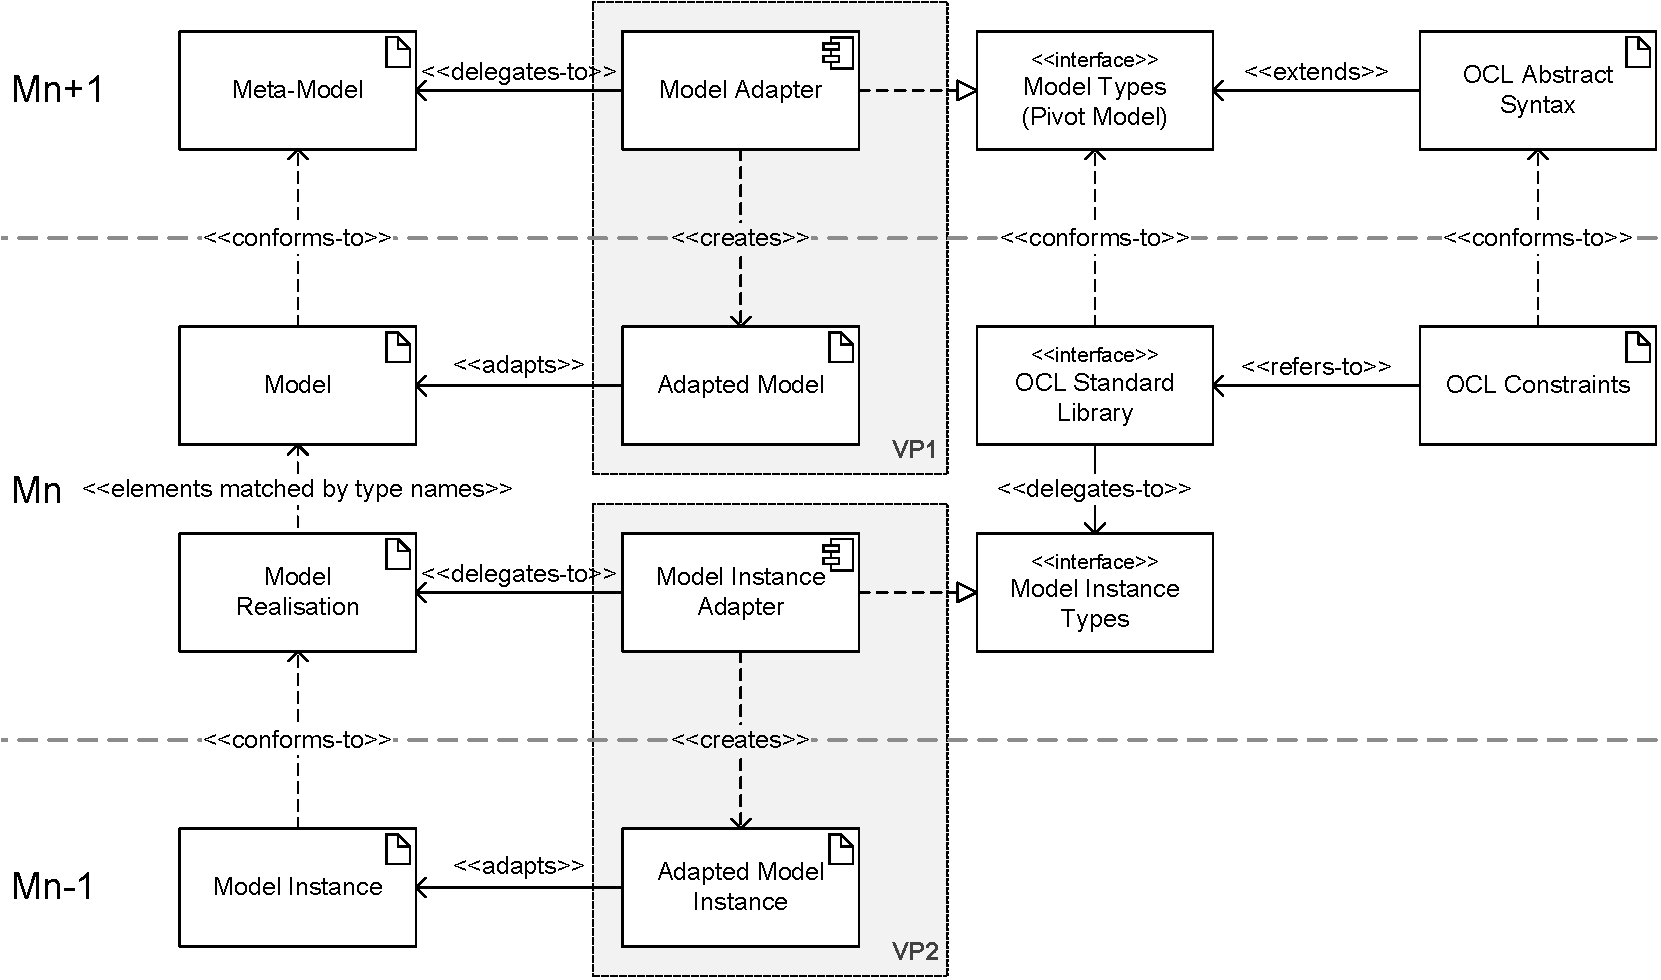
\includegraphics[width=1.00\textwidth]{figures/modeladaptation.pdf}
			\caption{The \emph{Generic Adaptation Architecture} of DresdenOCL: At the Mn+1 layer, meta-models are adapted
			to the model types (VP1). The model adapter component contains these adapters and is responsible 
			to instantiate them to adapt models of the meta-model. 
			At the Mn layer, model implementation types are adapted (VP2). The model instance adapter component
			contains these adapters and is responsible to instantiate them to adapt model instance objects. 
			The OCL standard library implements the logic to evaluate operations defined on OCL types. Other 
			requests such as operation invocations or property requests on adapted objects are delegated 
			via the interfaces of the model implementation type model.}
			\label{fig:modeladaptation}
		\end{figure}

	To enable the definition of OCL constraints for various modelling languages,
	DresdenOCL provides a set of common interfaces abstracting structures
	that are required to navigate and query object structures.
	These interfaces--called \emph{Model Types} (or \emph{Pivot Model}) \cite{braeuerOCL07}--standardize
	the basic	concepts such as types, properties, operations and parameters
	that bind OCL constraints to a concrete modelling language (cf. Fig. \ref{fig:coreconcepts}).
	DresdenOCL only	uses these concepts to parse and statically analyse OCL constraints, 
	e.g., the OCL2 parser	invokes the operation \texttt{getType()} to access the \texttt{Type} of 
	an \texttt{Operation} or \texttt{Property}.
	
	For every meta-model that shall be connected with DresdenOCL, 
	a \emph{Model Adapter} component has to be implemented (cf. Fig. \ref{fig:modeladaptation}, Mn+1 layer). 
	It contains individual adapters that map concepts of the modelling
	language to corresponding artefacts of the model types. E.g., the UML
	meta-model concept \texttt{UMLClass} is adapted to the model type concept
	\texttt{Type} \note{Christian: Again, figure needed. Claas: Fig 2 sufficient?}. 
	Furthermore, the model adapter component has to provide a factory to create 
	adapters on demand resulting in an \textit{Adapted Model} (cf. Fig.
	\ref{fig:modeladaptation}, Mn+1 and Mn layer).
	The adapters are only created for model elements that are required and
	existing adapters are cached. Thus, we avoid unnecessary and expensive adaptation, 
	especially when working on large models of which only parts are constrained using OCL.
	The presented architecture provides a generic and easy variation of multiple meta-models
	and corresponding models in an OCL infrastructure (VP1).


\subsection{Model Instance Adaptation}
	
	The presented abstraction of model types to support various models
	and meta-models can now be shifted and extended to
	solve similar problems when working with multiple model instantiations. Now we
	present the solution addressing the second variation point (VP2) for a generic adaptation
	architecture of an OCL infrastructure.
	
	Similar to the adaptation of different meta-models and models, it is
	useful to hide different model implementations
	behind standardised interfaces. This enables the
	reuse of the same OCL2 interpreter for the dynamic
	evaluation of OCL constraints on model instance elements in various model
	instantiations. To provide means for model
	instance adaptation, we introduced the \emph{Model Instance
	Types}. The model instance types are different
	interfaces for instances of standard types in OCL such as primitive types, 
	collections and objects (cf. Fig. \ref{fig:coreconcepts}). 
	All these	interfaces inherit a common interface \texttt{ModelInstanceElement}. The most 
	important difference between the model types and the model instance types
	is that \texttt{ModelInstanceElements} provide a reflection mechanism whereas 
	model type elements only allow to reason on relationship between concepts of
	the same meta-level. During interpretation, the OCL2 interpreter uses these reflection mechanisms to
	retrieve the \texttt{Type} of a \texttt{ModelInstanceElement}, access \texttt{Property}
	values, or to invoke \texttt{Operations}.
	
	Each kind of model instance that shall be connected with DresdenOCL is
	adapted via a \emph{Model Instance Adapter} component (cf. Fig.
	\ref{fig:modeladaptation}, Mn layer). Similar to the model adapter, 
	the model instance adapter component contains adapters that map elements of a
	concrete model instance to model instance types and has to
	provide a factory that creates \emph{Model Object Adapters} for the runtime 
	objects of the adapted model instance (cf. Fig. \ref{fig:modeladaptation}, Mn-1 layer). 
	Like the model adapter, the model instance adapter also 
	creates adapters for objects on demand. Adapted objects are cached to
	improve the performance and to avoid phenomena like \emph{Object
	Schizophrenia} \note{reference}. Due the introduction of a common set of model
	instance types it is possible to easily reuse the same OCL interpreter
	for various kinds of model instances. Thus, VP2 can be completely addressed
	by the presented generic adapter architecture.




  \section{Case Studies}

In this section we present three case studies to demonstrate the power of the presented
generic adaptation architecture.


\subsection{The Royal and Loyal System Example}

As a first case study, we modelled and implemented the \textit{Royal and Loyal System Example} 
as defined in \cite{warmer:ocl}. The case study was designed by \textsc{Warmer and Kleppe} to explain 
the Object Constraint Language and can be used to test the interpretation of
various kinds of OCL expressions. The case study consists of 13 UML classes (including inheritance and enumeration types)
and 130 constraints. We modelled the royal and loyal system using the UML2 meta-model of the
Eclipse Model Development Tools (MDT) project \cite{WWW:MDT}.
The model was implemented and instantiated in Java. Consequently
constraints were evaluated on Java objects.

\begin{figure}[!t]
	\centering
		\includegraphics[width=0.60\textwidth]{figures/casestudy01.pdf}
	\caption{In the Royal and Loyal case study, VP1 is bound to the \textit{MDT UML2 Model Adapter}. 
	  Consequently, the Royal and Loyal UML class diagram is adapted as a model at M1.
	  VP2 is bound to the \textit{Java Model Instance Adapter} and thus, each object of the Java 
	  implementation is adapted as a model instance object at M0.}
	\label{fig:casestudy01}
\end{figure}

The required adaptations for the royal and loyal case study are shown in Fig. \ref{fig:casestudy01}.
To parse the Royal and Loyal constraints
in DresdenOCL, a \textit{UML2 Model Adapter} component was implemented, that 
adapts the required meta-model elements from the MDT UML2 meta-model to the model 
types of DresdenOCL at the M2 layer and creates instances of these adapters for all UML models 
loaded into DresdenOCL. 
Consequently, the royal and loyal class diagram was adapted as a model at the M1 layer.
For the Java implementation, a \textit{Java Model Instance Adapter} component was implemented,
that adapts the Java meta-model elements (classes of the package \texttt{java.lang.reflect})
to the model instance types and creates instances of these adapters for all Java objects
loaded into DresdenOCL. Consequently, the objects of the royal and loyal Java implementation
were adapted as \texttt{ModelInstanceElements} in DresdenOCL at the M0 layer. Both, classes from 
the class diagram and from the Java implementation are located at the M1 layer 
because the Java classes are only other representations of the classes described by the 
UML class diagram! 

The Royal and Loyal case study demonstrates that our generic adapter architecture is able to 
support the common interpretation of OCL constraints defined on UML classes for Java objects.


\subsection{SEPA Business Rules}

As a second case study we tried to adapt our generic adaptation architecture to the
area of XML-structured data. Thus, we decided to interpret OCL consistency constraints
defined on an \textit{XML Schema Definition (XSD)} for an XML instance of this schema in a real, economy-driven
scenario. The company \textsc{Nomos Software} provides a service to check business rules on
financial \textit{Single Euro Payments Area (SEPA)} messages that are 
used in financial transactions of bank offices as defined by the \textit{European
Payment Council (EPC)}, \textit{ISO20022}, and the \textit{Euro Banking Association (EBA)} \cite{spec:UNIFI,spec:EPC}. 
SEPA messages are described and shipped as XML documents.
\textsc{Nomos Software} uses OCL constraints defined on XML schemas
to validate XML documents against a set of business rules that constrain the consistency of
this SEPA messages. We implemented an XSD model and an XML model instance adaptation 
for DresdenOCL and used the XSD and XML files that are 
provided with an online demo of the Nomos service for \textit{Pain.008.001.01} SEPA 
messages.\footnote{http://www.nomos-software.com/demo.html}
We took the about 120 constrains provided by the demo to test our adaptation. 

\begin{figure}[!t]
	\centering
		\includegraphics[width=0.60\textwidth]{figures/casestudy02.pdf}
	\caption{In the SEPA case study, VP1 is bound to the \textit{XSD Model Adapter}. 
	  Consequently, the Pain.008.001.01 schema is adapted as a model at M1.
	  VP2 is bound to the \textit{XML Model Instance Adapter} and thus, each node of the XML
	  instance is adapted as a model instance object at M0.}
	\label{fig:casestudy02}
\end{figure}

The required adaptations for the SEPA case study are shown in Fig. \ref{fig:casestudy02}.
To parse the SEPA constraints
in DresdenOCL, an \textit{XSD Model Adapter} component was implemented, that 
adapts the required meta-model elements from the XSD meta-model to the model 
types of DresdenOCL at the M2 layer and creates instances of these adapters for all XML schemas 
loaded into DresdenOCL. 
Consequently, the \textit{Pain.008.001.01} XML schema was adapted as a model at the M1 layer.
For the XML instances, an \textit{XML Instance Adapter} component was implemented,
that adapts the XML meta-model elements (mainly the class \texttt{org.w3c.dom.Node})
to the model instance types and creates instances of these adapters for all XML node instances
loaded into DresdenOCL. Consequently, the nodes of the Pain.008.001.01 XML messages
were adapted as \texttt{ModelInstanceElements} in DresdenOCL at the M0 layer.

These constraints of the Nomos service demo were evaluated for three different XML files 
and the results have been successfully compared with the results of the Nomos service demo.
This shows that our model implementation adaptation allows DresdenOCL to transparantly interpret
constraints on XML files as well. The OCL2 Interpreter had not to be modified for the SEPA case study!


\subsection{The OCL2.2 Standard Library}
The last case study depicts the ability to load different model instances of one model 
in order to check for inconsistencies between both instances. In this example we 
checked \textit{Well-Formedness Rules (WFRs)} for the OCL standard library of DresdenOCL. 
DresdenOCL's standard library is explicitly modelled as 
an instance of the model types, describing predefined OCL types like \texttt{Integer}, 
\texttt{OclAny} or \texttt{Sequence} and their associated operations. 
Hence, accessing predefined OCL types is reduced to a simple model 
import while the model can conveniently be queried, validated or altered 
\cite{braeuerOCL07}. The WFRs can be used to check whether all OCL types are 
declared and whether they support all operations that are defined by the 
current OCL specification.

Although modelling the standard library leads to great flexibility, the standard library 
still needs an implementation that provides its dynamic semantics. 
This implementation is provided through Java code. As the \textit{Model Types Editor} of Dresden OCL
does not support code generation, this can lead to inconsistencies between 
the modelled standard library and the according Java interfaces.
We propose to use OCL to check that all modelled types have an equivalent Java 
interface and all modelled operations are also present in the Java interface. Furthermore, 
this approach allows us to check whether the standard library supports all operations that 
are defined in the current OCL standard.

\begin{figure}[!t]
	\centering
		\includegraphics[width=0.60\textwidth]{figures/casestudy03.pdf}
	\caption{In the standard library case study, VP1 is bound to the \textit{EMF Ecore Model Adapter}. 
	  Consequently, the EssentialOcl Ecore model is adapted as a model at M1.
	  VP2 is bound to the \textit{XMI Model Instance Adapter} and thus, each element of the modeled Standard Library
	  instance is adapted as a model instance object at M0.}
	\label{fig:casestudy03}
\end{figure}

\note{Claas: Probably alter this section according to the description in the other two case studies above.}
In order to evaluate the WFRs, the model types need to be loaded as a model (cf. Fig. 
\ref{fig:casestudy03}) \note{Claas: Model Figure!} via the \textit{Ecore Model Adapter}. Now, the modelled standard library 
can be loaded as an instance of the model types via the \textit{XMI Model Instance Adapter}. Thus, 
we are able to evaluate the WFRs for the standard library model and can prove the correct 
structure of it according to the current OCL specification. 
\note{Claas: Emphasize the model layers used for interpretation here. Big difference to case studies 1 and 2!}

\note{Claas: Do we really have to mention this lack. Lets talk about the interpretation results instead.}
In order to check for inconsistencies with the Java implementation, the Java interfaces 
for predefined OCL types have \add{to} be loaded with the \textit{Java Class Model Instance Adapter}. Then, the same WFRs 
used for the standard library model before can be checked for this instance. 
Unfortunately, the \textit{Java Class Model Instance Adapter} does not exist yet, but will be 
implemented in the near future.


\subsection{Future Case Studies}

For future case studies we plan to adapt meta-model and model implementations for web services (Meta-Model: WSDL, Model Implementation: \note{TODO}), static programming languages such as C\# (Meta-Model: UML2, Model Implementation: C\#), data bases (Meta-Model: SQL-DDL, Model Implementation: SQL). 


  
  \section{Lessons Learnt}
\label{sec:lessons}

  In this section we highlight some challenges we faced during the design
  and implementation of our generic adaptation architecture for DresdenOCL.
  We present solutions to these challenges and possible improvements.

	\paragraph{Type Matching}
	As models and model instances are only loosely 
	coupled, \texttt{Model\-Instance\-Elements} must be matched to a model type
	when they are imported into DresdenOCL (cf. Fig.~\ref{fig:genericlayers}~(a)). 
	Currently, this type matching is realised by a simple type name match (including the names of 
	their enclosing namespaces whenever possible). E.g., the Java class \texttt{Loyalty\-Account} is
	matched to the UML class \texttt{Loyalty\-Account} in the royal and loyal case study.
	This matching algorithm can be rather complex and often information that could be 
	used to improve the matching is hidden inside the adapters. E.g., when adapting an instance of an EMF 
	Ecore model, one could use the \emph{generator model} provided by Ecore to
	retrieve further type matching information. We plan to improve this process
	that is currently scattered over multiple classes of each model instance 
	adapter component by introducing type matching strategies that 
	can be implemented using the \emph{chain of responsibility} 
	pattern \cite{gamma:dp}. The chain could start by trying to match the 
	types using a model instance specific matcher and end by trying to 
	simply match the type names as currently done.
	
	\paragraph{Element Unwrapping}
	Another problem when using adapters for \texttt{model\-Instance\-Types} 
	is the unwrapping mechanism of adapted elements when invoking operations 
	on the \texttt{Model\-Instance\-Elements}. E.g., to invoke an operation of an adapted Java 
	object we require \texttt{java.lang.Objects} as parameters instead of 
	\texttt{Model\-Instance\-Elements}. This unwrapping mechanism is easy 
	for elements that have been adapted before, as they simply can be unwrapped 
	again. Unfortunately, during interpretation of OCL constraints, 
	new instances of primitive types or new collections can be created 
	by the standard library (e.g., when invoking the OCL operation \texttt{size()} on a collection that 
	returns an \texttt{Integer} instance). Thus, a 
	model instance adapter has to provide operations to reconvert 
	primitive types and collections into elements of the adapted model 
	instances. In some cases this can become rather complicated as 
	the adaptation between types of the instance and the \texttt{model\-Instance\-Types} interfaces has not to be bijective. For 
	example, Java \texttt{ints} and \texttt{java.lang.Integers} are 
	both mapped to \texttt{ModelInstaceIntegers}. During unwrapping, 
	the Java model instance adapter component has to reflect 
	whether the method to invoke requires an \texttt{int}, an 
	\texttt{Integer} or another Java integer-like type instance.
	The unwrapping mechanism of an adapted instance 
	can be considered as the most complicated and error-prone part 
	of the complete model instance adaptation.
	Fortunately, model instances providing only structural information do not
	need this unwrapping mechanism as operations do not exist at all.

	\paragraph{Automated Adapter Creation}
	The adaptation process of models and model 
	instances contains parts that are similar 
	for each adaptation and thus can be automated.
	To improve the model adaptation process, we developed a code generator 
	for the creation of model adapter components. The code 
	generator requires an annotated meta-model describing
	the relation of meta-model concepts to the \texttt{model\-Types} (e.g., the UML meta-class
	\texttt{Classifier} is annotated as a \texttt{Type}). 
	The code generator generates the skeleton code for all required 
	adapters that has to be completed manually.
	For the \texttt{model\-Instance\-Types}, such a code generator is currently 
	missing, but could be implemented as well.
	
	\paragraph{Adaptation Testing}
	We developed two generic JUnit test suites, 
	that can be used to test the adaptation of a model 
	or model instance, respectively. 
	The test suites are initialised with a model or model instance that
	contains all the adapted concepts that shall be tested.
	The test suites then check if all required methods to 
	retrieve \texttt{Types}, \texttt{Operations}, \texttt{Properties} for the variation point VP1 are implemented or if the reflection mechanism
	provided by VP2 is supported appropriately.
	These generic test suites helped us to ensure 
	that all existing adaptations behave in the same expected manner
	and to easily detect wrong adaptations of some elements.
	Furthermore, these test suites can be used to ensure the absence of specific
	bugs in all adaptations by adding new test cases if such a bug is detected in one of the adaptations.

  \section{Related Work}
MDT OCL, USE, BluePrint OCL, AspectJ, ...

In \cite{hartmannDEXA06,hartmannICWI07} Hartmann presented an approach for XML-based template engines that showed a use case for OCL constraints on XML Schemas. OCL was used to express constraints that cannot be defined in XML Schema.

OCL on XML/DTD:
\begin{itemize}
	\item http://lci.cs.ubbcluj.ro/ocle/
	\item Modeling XML applications with UML (D. Carlson) (Buch)
\end{itemize}

\textbf{TODO}

  \section{Conclusion}

\begin{itemize}
  \item Conclusion:
  \begin{itemize}
    \item exchangability
    \item execution layer can be reused as well
    \item less errors, only one implementation, well tested
  \end{itemize}  
\end{itemize}

\section{Acknoledgements}

We want to thank Tricia Balfe of Nomos Software for providing their data for the XML case study and for continous feedback during adaptation of the case study.

\textbf{TODO} 

  \bibliographystyle{splncs}

  \bibliography{models2010}  

\end{document}
